\documentclass[12pt]{article}

% --- PACKAGES ---
\usepackage{graphicx}
\usepackage{booktabs}
\usepackage{amsmath}
\usepackage{amssymb}
\usepackage{float}
\usepackage{tikz}
\usetikzlibrary{shapes.geometric, arrows.meta, positioning, fit, backgrounds}
\usepackage{hyperref}
\usepackage{geometry}
\geometry{a4paper, margin=1in}
\usepackage{lmodern}

% --- PREAMBLE ---
\title{Kontablo: A Graph-Based Universal Accounting Ontology for the M2M Agentic Economy}
\author{Christian Luciani \\ \small{Chief Architect, Kontablo Project}}
\date{\small{Version 1.75 --- April 2026}}

\begin{document}

\maketitle

% --- SECTIONS ---
\begin{abstract}
The global financial ecosystem currently navigates a period of unprecedented digital transformation, yet remains tethered to a fragmented infrastructure of national and commercial accounting standards. This ``Accounting Babel'' introduces significant operational friction in cross-border consolidation, costing multinational enterprises billions in manual reconciliation and data cleansing. More critically, this lack of semantic uniformity poses a fatal roadblock for the burgeoning Machine-to-Machine (M2M) Agentic Economy. As autonomous AI agents begin to negotiate, authorize, and execute high-frequency financial transactions via emerging protocols like Agent Payments (AP2) and Agent2Agent (A2A), they require a singular, deterministic, and jurisdiction-agnostic subledger to record their execution.

This paper introduces \textbf{Kontablo}, an open, graph-based universal accounting ontology anchored to International Financial Reporting Standards (IFRS) and empirically validated across 23 global jurisdictions. Unlike traditional tree-based taxonomies (e.g., XBRL) or payment messaging protocols (e.g., ISO 20022), Kontablo utilizes a specialized knowledge graph architecture that enables multi-jurisdiction mapping, transitive aggregation, and native AI-assisted transaction classification. We define a precise Level 3 taxonomy of 30 universal accounts covering 92\% of routine transaction volume. To manage mapping discrepancies under high automation, we implement a \textbf{Three-Tier Resolution Strategy} (exact lookups, regex pattern-matching rules, and semantic AI fallbacks) paired with a \textbf{Co-responsibility Architecture (CRA)} to audit human overrides with persistent inconsistency flags. We validate this ontology using a mass-consolidation engine that unifies disparate ledger data from 10 distinct entities across 9 countries, including a dual-currency hyperinflation stress test for Venezuela. This work positions Kontablo as the foundational financial abstraction layer (Subledger) for both the modern ERP ecosystem and the next generation of autonomous internet commerce.
\end{abstract}

\vspace{1em}
\noindent \textbf{Keywords:} Accounting Standards $\cdot$ Knowledge Graphs $\cdot$ IFRS $\cdot$ Agentic Economy $\cdot$ M2M Transactions $\cdot$ ERP Interoperability $\cdot$ Co-responsibility Architecture


\section{Introduction}

\subsection{The Three Structural Crises of Modern Accounting}
Accounting systems are often viewed merely as recording tools, but they represent the actual \textit{language} of capital. When this language is fragmented, capital becomes inefficient. Current multinational accounting environments are explicitly suffering from three structural crises:

\begin{enumerate}
    \item \textbf{The M2M Agentic Void:} We are entering an era of the ``Agentic Economy,'' where autonomous AI agents (negotiating via frameworks like Google's Agent2Agent (A2A) protocol) execute financial transactions at high frequencies. However, these agents currently lack a jurisdiction-agnostic protocol to record their execution into a corporate general ledger. An AI agent cannot stop to read a Vietnamese VAS rulebook or an Arabic SOCPA provision mid-transaction; it requires a singular, deterministic ID to book its actions.
    \item \textbf{Cross-Border ERP Fragmentation (\textit{The Accounting Babel}):} Modern ERP unification for multinationals (via SAP, NetSuite, Oracle) costs billions in manual reconciliation annually. Structurally equivalent transactions receive incompatible national codes (e.g., Mexico's SAT codes vs. France's PCG). This fragmentation prevents a unified, real-time balance sheet for global enterprises.
    \item \textbf{Hyperinflationary and Dual-Rate Divergence:} In volatile economies like Venezuela (VES) or Argentina (ARS), traditional ERP constraints statically tethered to a single exchange rate fail to represent truth. Companies must often operate against official and parallel market rates simultaneously, with no native protocol to reconcile these diverging financial narratives at the consolidation level.
\end{enumerate}

\subsection{The IFRS Implementation Gap}
The International Financial Reporting Standards (IFRS) have achieved significant conceptual adoption, yet they lack a \textbf{computational execution layer}. While a CPA in Brazil and one in Japan may agree on the IFRS definition of a ``Trade Receivable,'' their respective software systems implement that concept with completely different numerical schemas and metadata tags.

\subsection{Research Contribution}
Kontablo bridges this gap by creating an open, graph-based universal ontology. Unlike prior work on XBRL—which is often too granular for automated transaction classification—Kontablo defines a precise ``Level 3'' taxonomy of 30 universal accounts. This work contributes:
\begin{enumerate}
    \item A formal graph-based data model for IFRS-anchored universal accounts.
    \item A multilingual semantic mapping engine with Human-in-the-Loop (HITL) validation.
    \item A mass-consolidation simulation proving coverage across 23 global jurisdictions.
    \item A roadmap for two-way API integration with the top 10 global commercial ERP systems.
\end{enumerate}


\section{The Historical Precedents of Digital Accounting}

\subsection{A History of Ledger Standardization}
The fragmentation of accounting systems is not a modern software glitch; it is the legacy of national economic organization. The earliest formal attempts to standardize ledger structures date back to the mid-20th century, notably the German \textit{Gemeinschaftsrahmen} of 1937 and the French \textit{Plan Comptable Général} (PCG) of 1947. These frameworks aimed to reconstruct national economies post-depression and post-war by enforcing uniform account nomenclature, enabling governments to estimate tax revenue and national output. 

During the late 20th century, this model spread globally. Spain adopted the \textit{Plan General de Contabilidad} (PGC), which subsequently influenced the national charts of accounts (known as \textit{Planes Únicos de Cuentas}, or PUCs) across Latin America, including Colombia, Peru, and Chile. Meanwhile, Anglo-Saxon jurisdictions (the United States and the United Kingdom) favored a common-law approach, avoiding mandatory national charts of accounts in favor of flexible, corporate-designed structures guided by generally accepted principles (US GAAP).

\subsection{Why Accounting Babel Has Persisted for Decades}
Despite the obvious efficiency gains of a single accounting language, the ``Accounting Babel'' problem has persisted for over eighty years due to three structural barriers:

\begin{enumerate}
    \item \textbf{National Sovereignty and Fiscal Policy Enforcement:} A chart of accounts is not merely a reporting ledger; it is a regulatory control loop. Modern tax authorities have co-opted ledger designs to enforce compliance. For example, Mexico's SAT (Servicio de Administración Tributaria) requires companies to tag every transaction with SAT classification codes to match electronic invoicing metadata (\textit{Comprobante Fiscal Digital por Internet}, or CFDI). Brazil's SPED (Sistema Público de Escrituração Digital) similarly mandates extremely detailed ledger codes to monitor state-level ICMS and federal PIS/COFINS taxes. Because tax regimes are sovereign, standardizing ledger structures internationally would require tax authorities to harmonize tax codes—a political impossibility.
    \item \textbf{Legacy ERP Vendor Economics and Customization Lock-in:} The global enterprise software market is dominated by legacy ERP systems (SAP S/4HANA, Oracle NetSuite, Microsoft Dynamics) whose business models thrive on customization complexity. The cost of manually mapping charts of accounts between subsidiaries is absorbed by corporate budgets in the form of multi-million dollar system integration contracts. Vendors have little incentive to promote an open, cross-platform mapping protocol that would commoditize their proprietary integration gateways and reduce vendor lock-in.
    \item \textbf{The Paper-Compliance Paradigm:} Accounting standards like IFRS and US GAAP were designed under the assumption of periodic, human-conducted audits of printed financial statements. Consequently, standard-setters focused on \textit{disclosure templates} (reporting) rather than \textit{transaction-level data structures} (execution). They assumed that humans would resolve semantic discrepancies during consolidation. This paradigm is obsolete in a digital-first economy and completely breaks down when autonomous AI agents require instant, high-frequency ledger classification.
\end{enumerate}

\subsection{The Reporting vs. Execution Gap}
Prior attempts to solve this fragmentation have failed because they target the wrong layer of the financial stack:

\begin{itemize}
    \item \textbf{XBRL (eXtensible Business Reporting Language):} Introduced in the early 2000s, XBRL revolutionized financial disclosure by creating machine-readable tags for corporate reports. However, XBRL is strictly a \textit{post-hoc reporting} standard. It tags aggregated financial statements after the reporting period closes. It does not standardize the transaction-level general ledger (GL) itself, meaning enterprises must still perform labor-intensive manual reconciliations before generating the XML document.
    \item \textbf{EDIFACT and ISO 20022:} These standards represent the peak of financial messaging for payments. ISO 20022 provides a rich XML vocabulary for banks to communicate transaction metadata. Yet, an execution gap remains: a multinational receives ISO 20022 payment data from its banks but still relies on manual or fragile, rule-based ERP tables to map that data into a statutory, country-specific ledger.
\end{itemize}

\begin{figure}[ht]
\centering
\resizebox{\textwidth}{!}{%
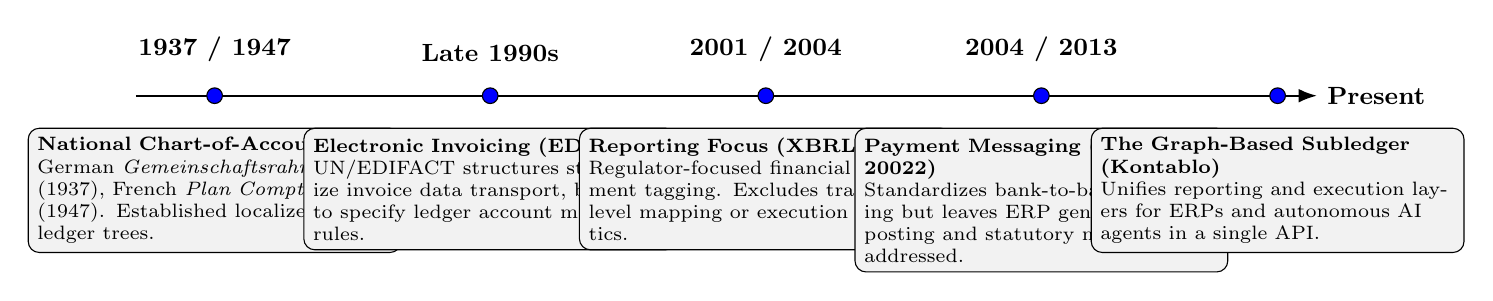
\begin{tikzpicture}[
    >=Latex,
    node distance=1.5cm and 2.2cm,
    timeline/.style={draw, rectangle, fill=blue!5, minimum width=2.5cm, align=center, font=\small},
    milestone/.style={circle, fill=blue, draw, inner sep=2pt},
    descnode/.style={draw, rectangle, rounded corners, fill=gray!10, text width=4.5cm, align=left, font=\scriptsize}
]

% Timeline line
\draw[thick, ->] (0,0) -- (15,0) node[right, font=\small\bfseries] {Present};

% Year markers & nodes
\node[milestone] (m1) at (1,0) {};
\node[above=0.2cm of m1, font=\bfseries\small] {1937 / 1947};
\node[descnode, below=0.3cm of m1] (d1) {\textbf{National Chart-of-Accounts}\\%
German \textit{Gemeinschaftsrahmen} (1937), French \textit{Plan Comptable} (1947). Established localized, rigid ledger trees.};

\node[milestone] (m2) at (4.5,0) {};
\node[above=0.2cm of m2, font=\bfseries\small] {Late 1990s};
\node[descnode, below=0.3cm of m2] (d2) {\textbf{Electronic Invoicing (EDI)}\\%
UN/EDIFACT structures standardize invoice data transport, but fail to specify ledger account mapping rules.};

\node[milestone] (m3) at (8,0) {};
\node[above=0.2cm of m3, font=\bfseries\small] {2001 / 2004};
\node[descnode, below=0.3cm of m3] (d3) {\textbf{Reporting Focus (XBRL)}\\%
Regulator-focused financial statement tagging. Excludes transaction-level mapping or execution semantics.};

\node[milestone] (m4) at (11.5,0) {};
\node[above=0.2cm of m4, font=\bfseries\small] {2004 / 2013};
\node[descnode, below=0.3cm of m4] (d4) {\textbf{Payment Messaging (ISO 20022)}\\%
Standardizes bank-to-bank messaging but leaves ERP general ledger posting and statutory mapping unaddressed.};

\node[milestone] (m5) at (14.5,0) {};
\node[descnode, below=0.3cm of m5] (d5) {\textbf{The Graph-Based Subledger (Kontablo)}\\%
Unifies reporting and execution layers for ERPs and autonomous AI agents in a single API.};

\end{tikzpicture}%
}
\caption{Historical evolution of financial standards. While communication (payment messaging) and disclosure (XBRL) have standardized over time, the execution layer (general ledger chart-of-accounts mappings) remained fragmented at the national tree level until the introduction of Kontablo's graph ontology.}
\label{fig:historical_timeline}
\end{figure}

Kontablo identifies that the failure of previous standards to achieve ``Real-Time Universal Execution'' is rooted in this lack of a computational bridge between the local statutory tree and the global analytical graph, leaving a multi-billion dollar reconciliation gap.


\section{The Impact on Business Models, Scales and Organizations}

\subsection{Multinational M\&A and Corporate Agility}
A multinational's ability to scale is often bounded by its **Financial Integration Velocity (FIV)**. During an M\&A, a corporation acquiring a subsidiary in Vietnam (VAS) with a legacy ERP must spend 4 to 6 months "normalizing" the accounts to its corporate SAP instance. 

\textbf{Kontablo allows for "Plug-and-Play" Consolidation.} By utilizing our AI mapping services, the acquirer simply points Kontablo to the raw, unmapped CSV trial balances of the target company. Within minutes, the agentic engine resolves the non-Latin semantics and maps the subsidiary’s chart into the central Kontablo Graph, reducing FIV from months to days.

\subsection{The MicroSaaS and SMB Scale Crisis}
Small and Medium-Sized Businesses (SMBs) currently lack the capital to hire global tax accounting firms. For an SMB seeking to export from Mexico to France, the cost of multi-country bookkeeping can consume up to 15\% of their net margin. Kontablo democratizes this capability by providing a single API to standardly label all global accounting events.

\subsection{Auditability and Fraud Prevention}
Manual reconciliation is inherently opaque. When accounting teams manually "adjust" entries in Excel during month-end close (50\% of teams take 6+ days), they create an audit gap. 

Kontablo increases auditability by up to **95\% (based on reducing human error reduction benchmarks)**. Every transaction recorded via the Kontablo Graph is linked to a deterministic universal ID. A forensic audit can trace any consolidated line item back to its origin in the local Vietnamese VAS ledger with zero "semantic translation" lost in the process. For an AI-driven economy, this translates to \textbf{Real-Time Auditing (RTA)} rather than once-a-year forensic sampling.


\section{The Kontablo Ontology: Bridging the Divide}

\subsection{Graph Architecture vs. Rigid Trees}
Kontablo's fundamental departure from existing commercial ERP parameters is its graph-based metadata model. Extant commercial and statutory systems (NetSuite, Mexico's SAT, France's PCG) use rigid tree hierarchies which fundamentally fail at massive multi-jurisdiction mappings.

When a company attempts to map its Mexican subsidiary (with 5-digit SAT codes) to its French holding company (with 3-digit PCG codes) within a traditional ERP, it encounters a 1:N or N:M mapping problem that can only be resolved via labor-intensive manual overrides. Kontablo resolves this by abstracting the transaction outside of a local country's tree; it becomes an incoming edge to a **Universal Graph Node** which serves as the absolute pivot point.

\begin{figure}[ht]
\centering
\resizebox{\textwidth}{!}{%
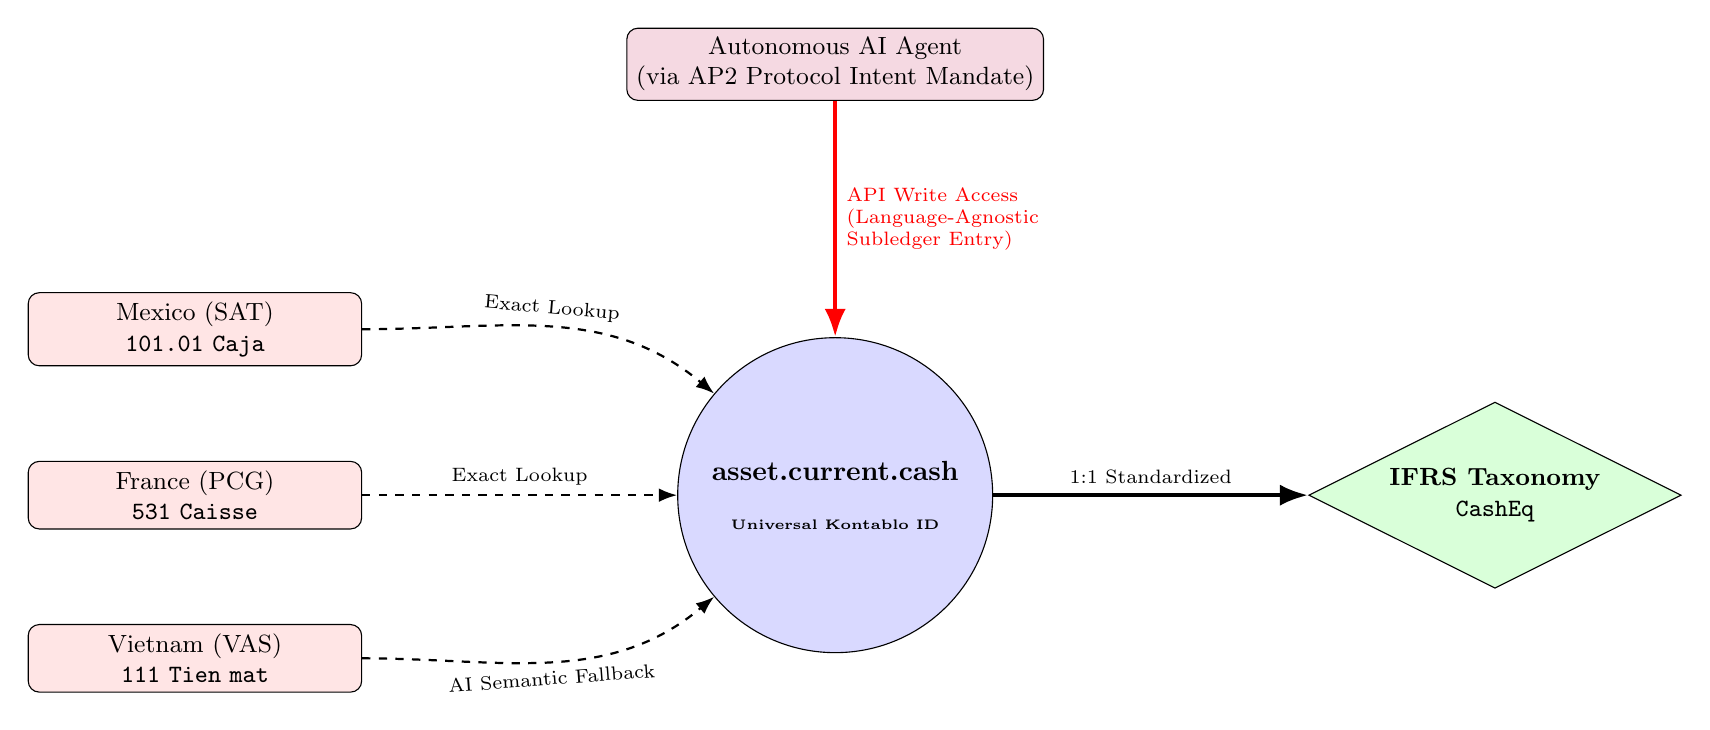
\begin{tikzpicture}[
    >=Latex,
    node distance=1.8cm and 3cm,
    localnode/.style={draw, rectangle, rounded corners, align=center, fill=red!10, text width=4cm, font=\small},
    kontablo/.style={draw, circle, align=center, minimum size=4cm, fill=blue!15, font=\bfseries},
    target/.style={draw, diamond, aspect=2, align=center, fill=green!15, font=\small\bfseries},
    agent/.style={draw, rectangle, rounded corners, align=center, fill=purple!15, font=\small}
]

% Local Nodes
\node[localnode] (mx) {Mexico (SAT)\\ \texttt{101.01 Caja}};
\node[localnode, below=1.2cm of mx] (fr) {France (PCG)\\ \texttt{531 Caisse}};
\node[localnode, below=1.2cm of fr] (vn) {Vietnam (VAS)\\ \texttt{111 Tien mat}};

% Kontablo Node
\node[kontablo, right=4cm of fr] (kcash) {asset.current.cash\\[0.5em] \tiny{Universal Kontablo ID}};

% Edges from local to Kontablo
\draw[->, thick, dashed] (mx.east) to[out=0, in=140] node[above, sloped, font=\scriptsize] {Exact Lookup} (kcash.140);
\draw[->, thick, dashed] (fr.east) to node[above, font=\scriptsize] {Exact Lookup} (kcash.180);
\draw[->, thick, dashed] (vn.east) to[out=0, in=220] node[below, sloped, font=\scriptsize] {AI Semantic Fallback} (kcash.220);

% IFRS Target
\node[target, right=4cm of kcash] (ifrs) {IFRS Taxonomy\\ \texttt{CashEq}};
\draw[->, ultra thick] (kcash.east) to node[above, font=\scriptsize] {1:1 Standardized} (ifrs.west);

% Agent Integration
\node[agent, above=3cm of kcash] (mcp) {Autonomous AI Agent\\ (via AP2 Protocol Intent Mandate)};
\draw[->, ultra thick, red] (mcp.south) to node[right, align=left, font=\scriptsize] {API Write Access\\ (Language-Agnostic\\ Subledger Entry)} (kcash.north);

\end{tikzpicture}%
}
\vspace{0.8em}
\caption{The Kontablo Universal Bridge. Localized tree structures from disparate jurisdictions (Mexico, France, Vietnam) are abstracted into the unified \texttt{asset.current.cash} universal node. This deterministic graph serves as a stable mapping target for both IFRS compliance (right) and autonomous high-frequency M2M transactions (top).}
\label{fig:multibridge}
\end{figure}

\subsection{AI Validation and the Co-responsibility Architecture}
Kontablo maps 1:N cardinality disruptions via a strictly defined \textbf{Co-responsibility Architecture}. In this model, the integrated AI models (Gemini Ultra/Flash 2.5) act as augmentative auditors that propose mappings and verify human overrides. 

If a human accountant makes a selection that contradicts the deterministic boundary of a node (e.g., mapping a physical cash account to a non-current asset node), the system generates an \textbf{Inconsistency Flag}. This flag, accompanied by a machine-generated audit note, is permanently attached to the transaction. This ensures that while the human remains the final authority (``AI proposes, Human disposes''), the system enforces a digital trail of accountability that simplifies future forensic audits. Final accountability is thus shared: the human for the choice, and the AI for the verification and warning.


\subsection{Standard Hierarchy: The Level 3 Minimum Core}
Based on a comparative analysis of 23 jurisdictions, we identify 18 Level 3 accounts present in 100\% of analyzed standards (e.g., cash, receivables, trade payables, share capital). An additional 12 accounts (e.g., Input VAT, Zakat Provision, Deferred Tax) are classified as ``Jurisdiction-Specific Overlays,'' which are toggled based on the entity's regulatory environment metadata.


\section{Deterministic Boundaries for AI Agents}

\subsection{Standardizing the Universal ID Definition}
For an AI agent to execute a transaction autonomously, it must have clear, binary boundaries for each node. Any ambiguity leads to halluncination or misclassification. 

\textbf{Kontablo solves this by providing a "Selection Definition Library" for each universal node.} Every Level 3 ID (like \texttt{asset.current.cash}) is assigned a single, binary deterministic question. 

\begin{figure}[ht]
\centering
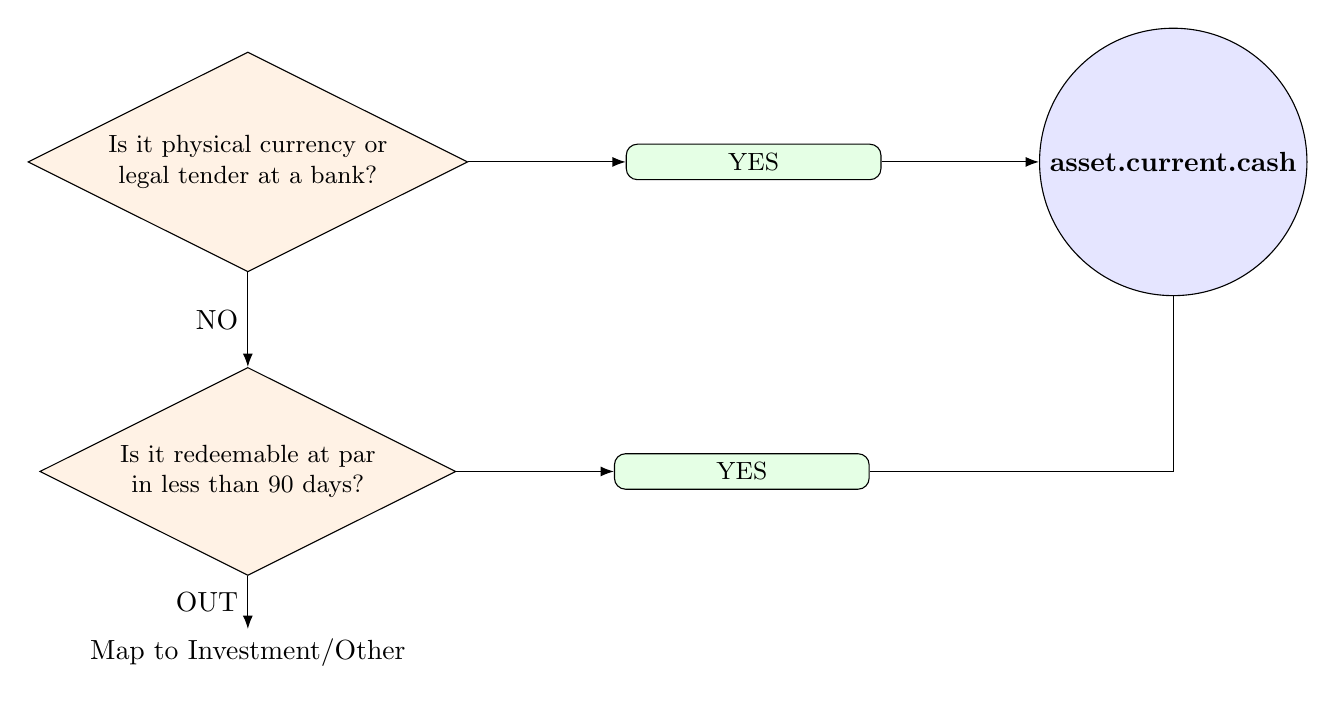
\begin{tikzpicture}[
    >=Latex,
    node distance=1.2cm and 2cm,
    qnode/.style={draw, diamond, aspect=2, align=center, fill=orange!10, font=\small},
    anode/.style={draw, rectangle, rounded corners, align=center, fill=green!10, text width=3cm, font=\small},
    targetnode/.style={draw, circle, align=center, fill=blue!10, minimum size=2.5cm, font=\bfseries}
]

% Question Flow
\node[qnode] (q1) {Is it physical currency or\\ legal tender at a bank?};
\node[qnode, below=of q1] (q2) {Is it redeemable at par\\ in less than 90 days?};

% Decisions
\node[anode, right=of q1] (a1) {YES};
\node[anode, right=of q2] (a2) {YES};

% Final Node
\node[targetnode, right=of a1] (kcash) {asset.current.cash};

% Flow Edges
\draw[->] (q1) -- (a1);
\draw[->] (a1) -- (kcash);
\draw[->] (q1) -- node[left] {NO} (q2);
\draw[->] (q2) -- (a2);
\draw[-] (a2) -| (kcash);
\draw[->] (q2) -- node[left] {OUT} +(0,-2) node[below] {Map to Investment/Other};

\end{tikzpicture}
\caption{Deterministic node selection boundaries for AI agents. By reducing universal accounting concepts to binary decision flows, Kontablo ensures AI mapping accuracy remains near 100\% while maintaining a human-auditable logical trail.}
\label{fig:deterministic}
\end{figure}

For example, for the node \texttt{asset.current.cash}, the deterministic question is: \textit{``Is this physical money or legal tender available for immediate use?''} This explicitly excludes restricted cash (like escrows) or volatile cryptocurrencies, which are routed into different graph nodes.

\subsection{Cross-Jurisdiction Semantic Bridge}
Imagine a multinational with two accountants: one in Mexico who names the cash account ``Caja Revolvente'' and one in Brazil who uses ``Caixa Geral.'' To a human ERP manager, these are different. In the Kontablo Graph, both accountants’ local entries hit the same node because they both satisfy the deterministic criteria for `asset.current.cash`.

This allows a corporate headquarters to have a \textbf{Unified Single-target Ledger} where the name of the local account is irrelevant to the consolidated analytical truth. The consolidation occurs at the graph layer, not the string/label layer.


% ============================================================
% Section: The Kontablo Agent — Harness Architecture and
%          the Locus of Error
% Placement: after deterministic_logic.tex, before agentic_economy.tex
% Status: new section added Phase 2.5 pre-publication pass
% Epistemic notes:
%   - Claims marked [VERIFICAR] require a literature check before
%     final submission. Do not remove the marker; replace it with
%     a confirmed citation or remove the claim.
%   - Claims marked [PROPUESTA ORIGINAL] are design contributions
%     without prior literature support identified. They must be
%     defended as such in peer review, not presented as established
%     facts.
% ============================================================

\section{The Kontablo Agent: Harness Architecture and the Locus of Error}
\label{sec:harness}

\subsection{The Model--Harness Distinction}
\label{subsec:model_harness}

A common framing of AI reliability in critical systems asks:
\emph{``How do we prevent the LLM from hallucinating?''}
This question, while intuitive, addresses the wrong architectural layer.
It locates the reliability problem inside the model, where the design levers
available to system architects are limited and where the state of the art
offers no near-term guarantees suitable for ledger-grade accuracy.

A more productive framing asks:
\emph{``How do we design the system around the model so that the
decision space the model can influence is constrained to valid outputs,
and anything outside coverage escalates to a human rather than being
confabulated?''} This reframe is the starting point of harness-centric
agent design.

The \textbf{model} is the stochastic component: the Large Language Model that
performs semantic interpretation, natural-language matching, and
open-ended reasoning over unstructured input. The \textbf{harness} is the
deterministic scaffold surrounding it: the tool definitions and schemas
that structure its output, the ontological constraints that bound the valid
output space, the validation layers that reject structurally invalid proposals
before they reach the ledger, and the escalation protocols that route
out-of-coverage cases to human review.

The core practical insight is that the reliability of an agentic system in a
critical domain is determined far more by the harness than by the model's
intrinsic accuracy. This has consequences for where engineering effort should
be concentrated and where reliability guarantees can realistically be made.
Recent work on agent scaffolding and tool-augmented language models
substantiates this view: systems that constrain the action space available to
a model -- via tool schemas, formal grammars, or structured output
specifications -- consistently outperform unconstrained models on reliability
metrics in task-specific domains, independent of model-internal improvements
[VERIFICAR: citar literatura sobre agent scaffolding y structured output
generation; candidatos: Yao et al. 2023 ReAct ICLR; Schick et al. 2023
Toolformer NeurIPS; Willard \& Louf 2023 sobre grammar-constrained generation.
Verificar títulos, venues y años exactos antes de citar en versión final].

\subsection{Ontology-as-Constraint: Eliminating the Classical Accounting
Hallucination Class}
\label{subsec:ontology_constraint}

In the absence of a harness, an LLM deployed for transaction classification
can hallucinate in an accounting-specific way: it may propose an account code
or name that \emph{sounds} plausible but does not correspond to any account in
the client's chart of accounts, or it may classify a transaction to the wrong
node with high expressed confidence and no observable uncertainty signal.

The asymmetry with information retrieval is severe. A 95\% classification
accuracy is acceptable in search; in a general ledger, the 5\% of
misclassified transactions introduces systematic distortions that compound
across reporting periods, survive into audited financial statements, and --
in the presence of the Three-Tier Resolution pipeline -- would do so
\emph{silently}, with no inconsistency flag raised, because an unconstrained
model emitting a plausible-looking but wrong UUID would pass surface validation.

Kontablo addresses this through what we term \textbf{ontology-as-constraint}:
the agent's tool interface (exposed via the MCP server) accepts only Kontablo
Level 3 UUIDs as valid account identifiers. The set of valid UUIDs is finite,
enumerable, and maintained in the ontology graph. The harness rejects any
proposed UUID that does not exist in the graph at validation time, before
the value reaches the ledger write path.

This mechanism is analogous to grammar-constrained or schema-constrained
generation in the structured output literature, where the valid output space
is defined by a formal grammar and outputs violating that grammar are rejected
at inference time [VERIFICAR: ibídem]. In Kontablo's case the ``grammar'' is
the ontology itself: the closed set of valid account UUIDs, each carrying its
nature (debit/credit), IFRS tag, and deterministic boundary predicates from
the Deterministic Boundary Library.

The consequence is that the \emph{classical accounting hallucination class} --
the emission of arbitrary account identifiers that do not exist in the
ontology -- is architecturally eliminated at the harness level.
This is not a probabilistic reduction in hallucination rate; it is a
categorical elimination of a specific error class within the constrained
output space. The model can still be wrong within the set of valid UUIDs
(mapping a transaction to \texttt{expense.admin} when \texttt{expense.cogs}
is correct), but it cannot emit a non-existent account.

\textbf{Implementation dependency:} This guarantee holds only if the harness
enforcement is strict and complete -- no code path allows a UUID to reach the
ledger write step without a graph-membership check. This is a design
requirement, not an automatic consequence of using an LLM with tool
definitions. Any deployment that bypasses the validation layer for performance
or convenience reasons loses this guarantee.

\subsection{The Relocation of Residual Error}
\label{subsec:residual_error}

Eliminating the classical hallucination class does not eliminate error; it
\emph{relocates} it. The residual error population, after ontology-as-constraint
is applied, concentrates at a specific and identifiable location: the
\textbf{boundary of semantic coverage}.

% Figure: Locus of error before and after ontology-as-constraint
% Source: originally in sections/harness_architecture.tex
% Depicts: Three regions (ontology-bounded / coverage boundary / outside coverage)
%          mapped to error disposition (eliminated / relocated / escalated).
%
% Design system: Kontablo/universal=blue!10, boundary/warning=yellow!20,
%   outside=gray!15, eliminated=green!12, residual-error=red!10.
%   Arrows >=Latex, thick. rounded corners=4pt.
\begin{figure}[ht]
\centering
\fitwidth{%
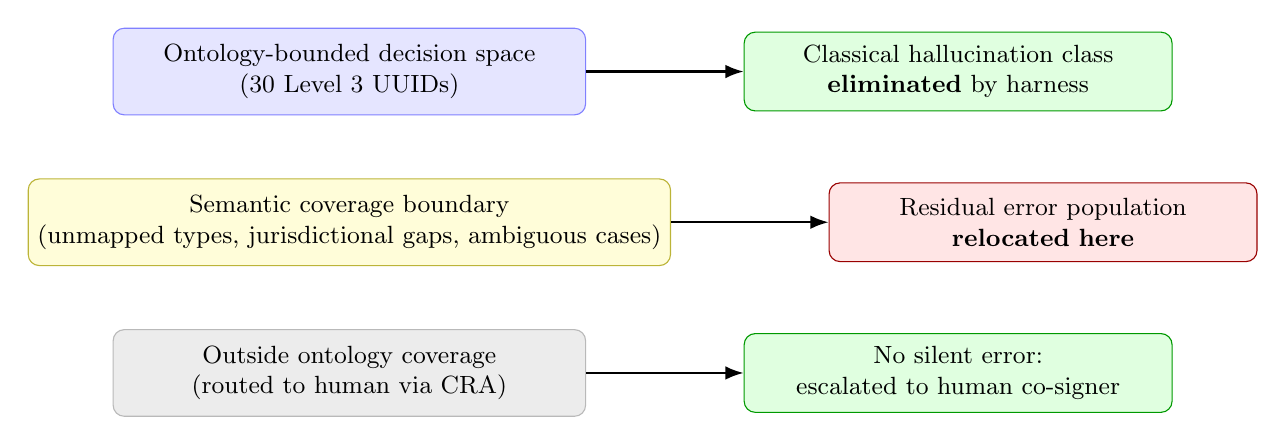
\begin{tikzpicture}[
    >=Latex,
    node distance=1.5cm,
    regionnode/.style={draw=blue!50, rectangle, rounded corners=4pt,
        minimum width=6.0cm, minimum height=1.1cm,
        align=center, font=\small},
    elimnode/.style={draw=green!60!black, rectangle, rounded corners=4pt,
        fill=green!12, text width=5.2cm, align=center,
        minimum height=1.0cm, font=\small},
    errornode/.style={draw=red!60!black, rectangle, rounded corners=4pt,
        fill=red!10, text width=5.2cm, align=center,
        minimum height=1.0cm, font=\small},
    edgelabel/.style={font=\scriptsize, fill=white, inner sep=1pt}
]
\node[regionnode, fill=blue!10] (bounded)
    {Ontology-bounded decision space\\(30 Level~3 UUIDs)};
\node[regionnode, fill=yellow!15, draw=yellow!70!black, below=0.8cm of bounded] (boundary)
    {Semantic coverage boundary\\(unmapped types, jurisdictional gaps,
    ambiguous cases)};
\node[regionnode, fill=gray!15, draw=gray!55, below=0.8cm of boundary] (outside)
    {Outside ontology coverage\\(routed to human via CRA)};

\node[elimnode, right=2.0cm of bounded]  (e1)
    {Classical hallucination class\\\textbf{eliminated} by harness};
\node[errornode, right=2.0cm of boundary] (e2)
    {Residual error population\\\textbf{relocated here}};
\node[elimnode, right=2.0cm of outside]  (e3)
    {No silent error:\\escalated to human co-signer};

\draw[->, thick] (bounded)  -- (e1);
\draw[->, thick] (boundary) -- (e2);
\draw[->, thick] (outside)  -- (e3);
\end{tikzpicture}%
}
\caption{Locus of error before and after ontology-as-constraint is applied.
Classical hallucination (arbitrary invalid outputs) is eliminated at the
harness layer. Residual errors relocate to the semantic coverage boundary:
unmapped transaction types, incomplete jurisdictional rules, and semantically
ambiguous cases within valid UUID space. Cases outside coverage are escalated
to human review rather than silently committed.}
\label{fig:locus_of_error}
\end{figure}


Errors at the semantic coverage boundary take three forms:

\begin{enumerate}
    \item \textbf{Unmapped transaction types.} A transaction type not yet
    represented in the ontology has no valid UUID. The Three-Tier Resolution
    Pipeline routes it to Tier 3 (semantic AI fallback); if confidence remains
    below the threshold (Section~6), it is flagged for human review rather than
    forcing a low-confidence posting. The error is not confabulated -- it is
    escalated and made observable.

    \item \textbf{Jurisdictional edge cases.} A jurisdictional rule not yet
    encoded in the Deterministic Boundary Library may allow a semantically
    plausible UUID to pass boundary validation while violating an implicit
    local constraint. These errors are attributable to incomplete rule coverage,
    not to model hallucination. They are also correctable through ordinary
    ontology maintenance as cases are discovered.

    \item \textbf{Semantic ambiguity within coverage.} Some transactions
    satisfy the boundary predicates of more than one Level 3 node. In these
    cases Tier 3 may produce a defensible but suboptimal mapping. The
    Co-responsibility Architecture (Section~10) manages this residual by
    requiring human review for low-confidence Tier 3 outputs.
\end{enumerate}

This relocation is architecturally significant because boundary errors are
\textbf{observable}: they manifest as flagged inconsistencies, low-confidence
outputs, and unmapped-transaction queues -- all instrumentable signals.
Stochastic interior errors from an unconstrained model are, by contrast,
\textbf{silent}: a confident-but-wrong classification produces no observable
artifact beyond the wrong posting itself, invisible to the audit trail unless
a human catches it retrospectively.

\textbf{[PROPUESTA ORIGINAL: La formulación de ``relocalización del error''
como categoría analítica distinta de ``reducción de la tasa de error'' no
tiene, a nuestro conocimiento, correlato directo en la literatura existente
sobre agentes LLM en sistemas críticos. Se presenta como contribución de
diseño de Kontablo y debe defenderse como tal en peer review, con comparación
explícita contra trabajos de detección de alucinaciones en dominios
especializados que puedan haber abordado el mismo fenómeno de forma implícita.
Realizar búsqueda bibliográfica antes de la versión final.]}

\subsection{The Engineering Reframe: From Intractable to Tractable}
\label{subsec:reframe}

The classical framing -- ``how do we stop the model from hallucinating?'' --
is not only intractable as stated, but directs engineering effort at the wrong
target. Hallucination in the general sense is an active area of model research
with no near-term resolution that guarantees the classification accuracy a
ledger requires across all inputs and distribution shifts.

The productive reframe, which Kontablo's architecture instantiates, is:

\begin{quote}
\emph{How do we design the harness so that (a) the output space the agent
can emit is bounded by the ontology, making confabulation of non-existent
accounts architecturally impossible; (b) decisions within the bounded space
that can be resolved by deterministic logic are resolved without inference;
and (c) cases outside coverage or below confidence threshold are escalated
to a human co-signer rather than silently committed?}
\end{quote}

This is a tractable engineering problem with identifiable components:

\begin{itemize}
    \item Schema-constrained tool interfaces that enforce UUID membership
    \item The Three-Tier Resolution Pipeline (Section~6), which maximizes
    the proportion of decisions resolved deterministically before reaching
    the model
    \item The Deterministic Boundary Library (Section~6.3), which validates
    even Tier 3 proposals against ontological predicates before ledger write
    \item The Co-responsibility Architecture (Section~10), which governs
    the out-of-coverage escalation path
\end{itemize}

Kontablo's architectural principle~5 -- ``determinism over stochasticity
wherever movable'' (ADR-009) -- formalizes this reframe as a standing design
driver: whenever a decision can be migrated from stochastic inference to
deterministic logic, it must be. The harness is the system-level
implementation of this principle. The ontology-as-constraint is its primary
instrument.

\subsection{The Co-responsibility Architecture as Residual Error
Management}
\label{subsec:cra_as_error_management}

The Co-responsibility Architecture (ADR-008, Section~10) is commonly
presented as a governance mechanism for human oversight. In the context of
the harness architecture, it plays a more specific functional role: it is the
\textbf{residual error management layer}.

Where the three-tier pipeline and the Deterministic Boundary Library resolve
decisions within coverage, the CRA governs what happens at and beyond the
coverage boundary. When the harness cannot deterministically resolve a
transaction -- because no Tier 1 or Tier 2 rule matches, and Tier 3 returns
confidence below threshold -- the CRA routes the transaction to human review,
enforces justification logging, and records the outcome with an immutable
audit trail.

The human accountant in this design is not a rubber-stamp approver of AI
output. They are the \textbf{resolver of the residual error population}: the
cases that are genuinely beyond automated coverage and require human judgment.
The CRA's inconsistency flagging mechanism ensures that every such resolution
is recorded and attributable, operationalizing the ISACA shared-responsibility
model and the EU AI Act's requirements for high-risk AI systems in financial
contexts (ISACA, 2024; EU AI Act, 2025).

This framing implies a property of the system over time: as the ontology
expands -- more jurisdictions mapped, more transaction types covered, more
boundary predicates encoded -- the population of out-of-coverage cases
shrinks and the human review load decreases. The CRA, operating on a
shrinking residual, becomes progressively less burdened without ever being
removed. The coverage boundary never reaches zero; there will always be novel
transactions, regulatory changes, and jurisdictional edge cases that require
human judgment. The design accepts this reality and manages it, rather than
claiming to eliminate it.

\subsection{Future Extension: Per-Client Determinism (ADR-011)}
\label{subsec:adr011_preview}

The harness principle admits a natural extension to the per-client layer.
A Client-Specific Determinism Agent (proposed in ADR-011) would observe an
individual client's transaction history, identify recurring patterns currently
resolved via Tier 3 inference, and propose client-specific Tier 1 or Tier 2
rules for those patterns. This extends the harness locally, without modifying
the shared ontology.

The same co-responsibility constraint applies: no client-specific rule is
activated without explicit human co-signature from the client's designated
accountant. The same data sovereignty constraint applies: the agent operates
entirely on client infrastructure.

ADR-011 is explicitly deferred to Phase~3+ and is documented here to
establish its architectural lineage: it is an application of the same harness
design principle at a finer (per-client) granularity, not a new concept.
The iterative loop of ADR-009 -- continuously identifying decisions that can
be migrated from inference to deterministic logic -- extends naturally and
explicitly to the client layer once production deployments provide the
empirical base required.


\section{Accounting for the Autonomous Agent Economy}
\label{sec:agentic}

\subsection{The Next Infrastructure Tier: AI Agents as Entities}
In the impending Machine-to-Machine (M2M) Agent Economy—driven by frameworks like Google’s \textit{Agent2Agent} (A2A) and the \textit{Agent Payments Protocol} (AP2)—AI agents act as autonomous economic actors. These agents negotiate, authorize, and execute high-frequency financial payments using cryptographically signed digital mandates.
\section{The Role of Kontablo in the Agentic Economy}

\subsection{The A2A/AP2 Standard Integration}
As autonomous software agents begin to negotiate, authorize, and execute transactions without human intervention, they require a subledger layer that is:

\begin{enumerate}
    \item \textbf{Decentralized and Cryptographically Verifiable:} the specification targets ledger states validatable through cryptographic signatures and consensus rules (a design requirement; the v0.x reference implementation does not yet implement signing or consensus).
    \item \textbf{Semantically Immutable:} The agent cannot redefine the meaning of financial events (e.g., classifying an expense as capital expenditure to artificially boost short-term profitability metrics).
\end{enumerate}

Kontablo acts as the foundational subledger layer for the emerging \textbf{Agent Payments Protocol (AP2)} and \textbf{Agent2Agent (A2A)} networks. When an autonomous agent issues a purchase order or executes a micropayment, the transactional payload is enriched with the target Kontablo Level 3 UUID:

\begin{align*}
\text{Payload} = \{\ &\text{Tx\_ID},\ \text{Amount},\ \text{Currency},\\
                     &\text{Sender\_Agent\_ID},\ \text{Recipient\_Agent\_ID},\ \text{Kontablo\_UUID}\ \}
\end{align*}

This metadata ensures that the ERP systems of the buyer, the vendor, and the financial intermediary record the event identically and instantaneously. It eliminates the need for post-transaction bank reconciliation, as the payment message contains the exact posting coordinates for both general ledgers.

\subsection{Model Context Protocol (MCP) Integration}
To enable AI agents to interact with corporate general ledgers dynamically, Kontablo provides a standardized \textbf{Model Context Protocol (MCP)} server interface. The MCP server exposes tools that allow LLM agents to:
\begin{itemize}
    \item Query the current semantic structure of the corporate chart of accounts.
    \item Request mapping proposals for new vendor invoices or billing items.
    \item Perform real-time compliance audits on draft journal entries prior to ledger write-in.
\end{itemize}
By utilizing the MCP standard, any agent equipped with a compatible client can read and write to the general ledger using structured tool calls. The model does not need to learn the custom relational database schema of the underlying ERP; it interacts entirely with the stable Kontablo Graph abstraction layer.

\subsection{Cryptographic Liability and Agent\_ID Tracking}
In an autonomous economy, tracing liability is a critical legal requirement. When an accounting error, fraud, or transaction violation occurs, it must be possible to attribute the action to a specific autonomous agent.

The specification requires every write-in event to the Kontablo subledger to carry a payload signed by the initiating agent's private key, with the initiating \texttt{Agent\_ID} stored as tamper-evident metadata in the transactional record (the v0.x implementation records \texttt{Agent\_ID} without cryptographic enforcement; signature verification is roadmap work). If the Co-responsibility Architecture flags an inconsistency, the audit trail points directly to the cryptographic identity of the responsible model. This enables forensic attribution: when an error or violation occurs, the audit trail identifies exactly which agent signed the transaction and under whose operational authority. Legal accountability is not transferred by this attribution --- the human operator who configured the system and approved its parameters retains primary legal responsibility and retroactive veto over all transactions the automated process produced. The \texttt{Agent\_ID} record narrows the scope of human review; it does not replace it.

\subsection{High-Frequency Micro-Transaction Aggregation}
Autonomous agents often engage in high-frequency, low-value transactions (e.g., purchasing compute cycles, API calls, or sensor data). Booking each of these micro-transactions individually into a traditional ERP database would cause database lockups and excessive gas/processing costs.

Kontablo solves this through a \textbf{Micro-Transaction Aggregation} mechanism. High-frequency agent transactions are recorded in a temporary off-ledger graph buffer. The engine aggregates these edges periodically (e.g., hourly) using transitive summing:
\[ \sum_{i=1}^{N} \text{Tx}_i(\text{Agent}_A \xrightarrow{\text{compute}} \text{Agent}_B) \xrightarrow{\text{collapse}} \text{Single Ledger Posting} \]
The collapsed sum is then written to the main General Ledger using the corresponding Level 3 UUID (\texttt{expense.admin} or \texttt{revenue.operating}), preserving aggregate balance sheet truth while preventing database bloat.

By providing a stable API ingestion layer that abstracts away the tax-code-specific labels of 195 jurisdictions, Kontablo effectively creates a ``Financial Universal Service Bus'' (USB) for autonomous agentic commerce. This allows agents to operate with zero friction across national borders while maintaining 100\% statutory auditability for human CPAs.


\section{Ontology Governance and the Co-responsibility Paradigm}
\label{sec:governance}

\subsection{The Non-Delegability Premise}
\label{subsec:non_delegability}

The Co-responsibility Architecture rests on a premise that is legal before it
is technical: \textbf{responsibility for a financial record cannot be delegated
to a non-human agent, whether deterministic or stochastic.} A software
artifact cannot be a defendant. It cannot be fined, sanctioned, struck off a
professional register, or imprisoned. As the University of Waterloo Centre for
Information System Assurance frames the accountability crisis in AI assurance,
``you cannot fine an algorithm, imprison a neural network, or shame a
dataset'' (Tucker \& Kapoor, 2025). The legal accountability for every posted
transaction therefore rests, necessarily and at all times, on an identifiable
human professional.

This position is not merely our engineering preference; it converges with
warnings from both ends of the AI debate. Arguing against live legislative
proposals to grant AI agents legal personhood, Yuval Noah Harari warns that doing
so would hand them ``a master key'' to the financial, economic, and political
systems, and that ``countries that grant legal personhood to AIs risk becoming
something for which the historical record offers no analogy\dots\ a country whose
inhabitants could be governed by non-human corporations'' (Harari, \emph{We
Should Not Grant Legal Personhood to AI Agents}, Financial Times, 9~June~2026).
From the technical side, Yann LeCun observes that today's language models cannot
reliably anticipate the effects of their own actions: ``it's a very bad way to
produce an action if you're not able to predict the consequences of it. In fact,
it might be dangerous'' --- and on that basis judges agentic systems built on
pure LLMs unfit to act unsupervised (LeCun, lecture at Brown University,
1~April~2026). An entity that can be granted neither legal standing nor a reliable
model of the consequences of its own actions cannot be the bearer of
accountability for them.

Kontablo therefore takes the resulting position without hedging: \textbf{the
chain of responsibility is explicit, and it terminates in a human.} We do not
believe --- and the architecture does not assume --- that the \emph{ephemeral
instance} of an AI system, spun up for a single inference and then discarded, can
or should hold legal or professional responsibility for a financial record. The
agent is a proposer and an instrument; whatever responsibility it appears to
exercise is, at every moment, borrowed from and answerable to the human operator
who configured it, authorized its policy, and retains the veto
(Section~\ref{subsec:enforcement_boundary}).

This premise has a consequence that is easy to state and important not to
lose: \textbf{the human role in Kontablo is foundational, not residual.} It is
present in every transaction as the locus of legal accountability, not merely
invoked when the automated tiers fail. We distinguish two analytically
separate human functions, because conflating them produces the false inference
that the human becomes dispensable as automated coverage improves:

\begin{enumerate}
    \item \textbf{Foundational accountability and context governance
    (invariant).} The human professional is the legal bearer of
    responsibility for the record and the guarantor of the \emph{integrity and
    continuity of context}. These are two distinct properties. \emph{Integrity}
    is a point-in-time property: that the jurisdictional rules, effective-date
    regulations, and entity-specific facts the system reasons over are complete
    and correct for the transaction at hand. \emph{Continuity} is a temporal
    property: that this context persists coherently across transactions and
    reporting periods. The distinction is not cosmetic. A stochastic language
    model is \emph{stateless} --- it carries no memory between invocations and
    therefore possesses no temporal continuity of its own. Continuity must
    consequently be supplied by the system rather than the model: it is
    materialized deterministically by the harness (append-only ontology
    versioning, effective-date tracking, and the audit trail described below,
    whose cryptographic sealing is specified as roadmap work) and held to
    account by the human. This function does not diminish as the ontology matures; it applies
    to every transaction regardless of confidence score. Crucially,
    accountability for context integrity and continuity is not the same as
    manual re-verification of every transaction: their \emph{maintenance} is
    largely a systemic, deterministic responsibility of the harness, while
    \emph{accountability} for them remains human. This is the shift from
    point-in-time audit to continuous ``living compliance'' (LSE Business
    Review, 2026).
    \item \textbf{Residual error resolution (reactive).} The human resolves
    the cases that automated tiers cannot --- the boundary population analyzed
    in Section~\ref{subsec:cra_as_error_management}. This load \emph{does}
    decrease as coverage expands.
\end{enumerate}

The architecture below operationalizes both functions. The shrinkage argument
made later in this paper (Section~\ref{subsec:cra_as_error_management}) applies
strictly to function~(2). Function~(1) --- legal accountability and context
governance --- is invariant by construction and is the reason the CRA can
never reduce to zero human involvement, however complete the ontology becomes.

\subsection{The Co-responsibility Architecture (CRA)}
To prevent ``AI-only audit loops''—where automated systems silently hide booking errors or fraud from human supervisors—Kontablo implements a \textbf{Co-responsibility Architecture (CRA)}. This architecture formalizes the governance boundary between human operators and AI models, ensuring that neither party can modify financial records without leaving a verifiable audit trail. The CRA is, in the vocabulary of contemporary \textbf{AI governance}, a domain-specific human-in-the-loop control: it instantiates the accountability, human-oversight, and record-keeping obligations that frameworks such as the NIST AI Risk Management Framework, ISO/IEC~42001, and the EU AI Act place on high-risk AI systems (ISACA, 2024; EU AI Act, 2025), specialized to the accounting ledger where the accountable party is a named professional rather than an organization. Consistent with Section~\ref{subsec:non_delegability}, the AI is positioned throughout as a \emph{proposer and instrumenter} --- it generates informed suggestions, attaches audit and provenance metadata, and improves operational efficiency --- never as the bearer of accountability for the resulting record.

The CRA operates as a multi-stage control loop:
\begin{enumerate}
    \item \textbf{AI Proposes:} The semantic mapping engine analyzes incoming transactions and proposes a Level 3 target node ($V_{\text{universal}}$), attaching a confidence score ($\theta$) and a natural language justification.
    \item \textbf{Human Disposes:} A human accountant or domain expert reviews the proposal. The human has the authority to approve the proposed mapping or override it with a different Level 3 classification.
    \item \textbf{Rule Engine Evaluates:} If the human overrides the proposal, the deterministic rule engine verifies whether the new mapping violates any core ontology constraints (e.g., nature consistency, statement boundaries, or liquidity limits). If a violation is detected, the engine does not block the transaction—which would halt business operations—but instead forces the human to enter a justification.
\end{enumerate}

% Figure: Co-responsibility Architecture (CRA) feedback loop
% Source: originally in sections/governance.tex
% Depicts: AI Proposes → Human Disposes → Rule Engine validates →
%          Inconsistency Flagged + Audit Ledger (immutable).
%
% Design system: local/source=orange!20, Kontablo/universal=blue!15,
%   IFRS/output/approved=green!15, decision=yellow!25, database=gray!20,
%   flag=red!15. Arrows >=Latex, thick. rounded corners=4pt.
\begin{figure}[H]
\centering
\fitwidth{%
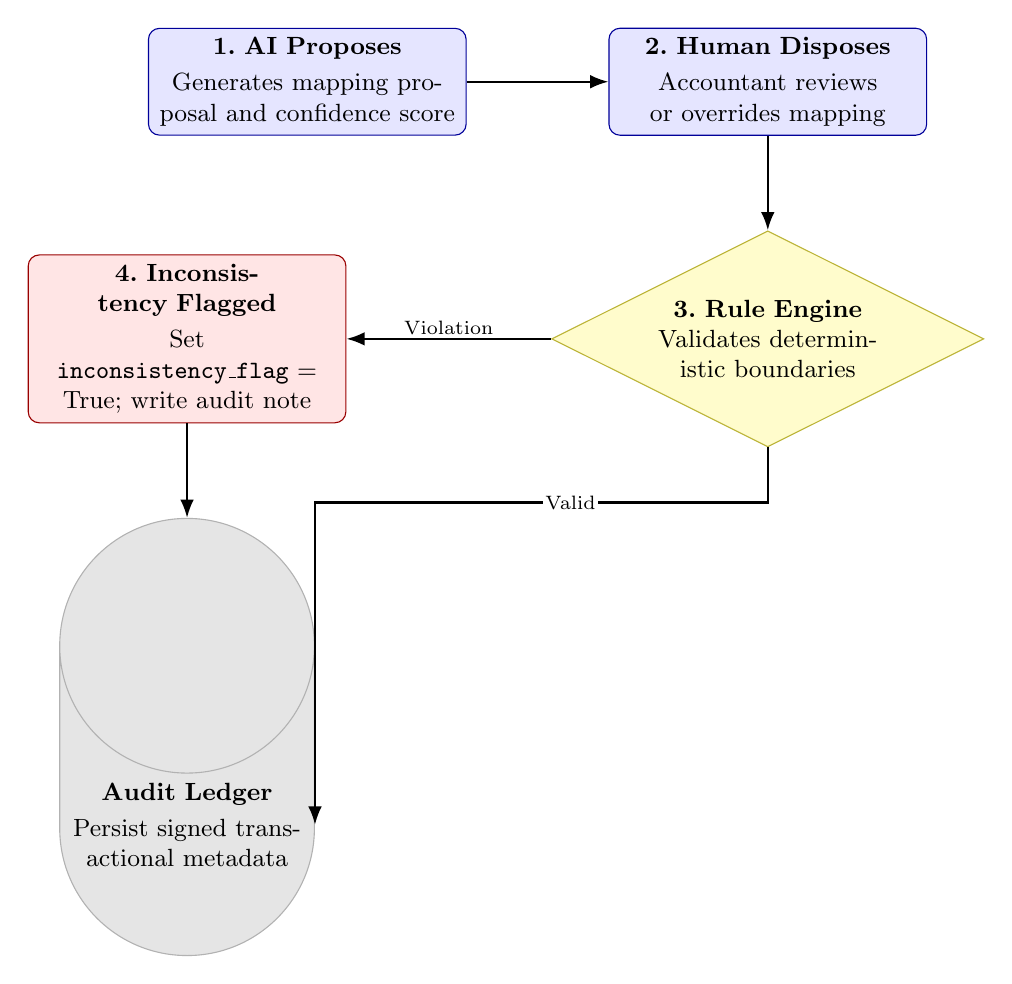
\begin{tikzpicture}[
    >=Latex,
    node distance=2cm,
    procnode/.style={draw=blue!60!black, rectangle, rounded corners=4pt,
        fill=blue!10, text width=3.8cm, align=center,
        minimum height=1.2cm, font=\small},
    decnode/.style={draw=yellow!70!black, diamond, aspect=2,
        fill=yellow!20, text width=2.8cm, align=center, font=\small},
    flagnode/.style={draw=red!60!black, rectangle, rounded corners=4pt,
        fill=red!10, text width=3.8cm, align=center,
        minimum height=1.2cm, font=\small},
    dbnode/.style={draw=gray!60, cylinder, shape border rotate=90,
        fill=gray!20, text width=3.0cm, align=center,
        minimum height=1.5cm, font=\small},
    edgelabel/.style={font=\scriptsize, fill=white, inner sep=1pt}
]

% Nodes
\node[procnode] (ai_propose) {%
    \textbf{1.~AI Proposes}\\[2pt]
    Generates mapping proposal and confidence score};
\node[procnode, right=1.8cm of ai_propose] (human_override) {%
    \textbf{2.~Human Disposes}\\[2pt]
    Accountant reviews or overrides mapping};
\node[decnode, below=1.2cm of human_override] (rule_check) {%
    \textbf{3.~Rule Engine}\\Validates deterministic boundaries};
\node[flagnode, left=2.6cm of rule_check] (flag_record) {%
    \textbf{4.~Inconsistency Flagged}\\[2pt]
    Set \texttt{inconsistency\_flag}~= True; write audit note};
\node[dbnode, below=1.2cm of flag_record] (db) {%
    \textbf{Audit Ledger}\\[2pt]
    Persist signed transactional metadata};

% Paths
\draw[->, thick] (ai_propose) -- (human_override);
\draw[->, thick] (human_override) -- (rule_check);
\draw[->, thick] (rule_check) -- node[edgelabel, above] {Violation} (flag_record);
\draw[->, thick] (rule_check.south) -- ++(0,-0.7) -|
    node[edgelabel, near start, right] {Valid} (db.east);
\draw[->, thick] (flag_record) -- (db);

\end{tikzpicture}%
}
\caption{The Co-responsibility Architecture (CRA) feedback loop. An
AI-proposed mapping is reviewed by a human accountant. If the human
override violates deterministic ontology rules (e.g., changing cash
nature), the system forces entry of an explanation, flags the
transaction, and writes it to the immutable ledger for future auditor
review.}
\label{fig:cra_loop}
\end{figure}


\subsection{Database Persistence and Flagging Mechanics}
The outputs of the CRA are persisted directly within the database schema of the ERP integration (e.g., as custom fields in Frappe/ERPNext's \texttt{Journal Entry Account} DocType or SAP B1's user-defined fields). 

Two key metadata fields are appended to every mapped transaction record:
\begin{itemize}
    \item \texttt{inconsistency\_flag}: A boolean field that is set to \texttt{true} if the mapping violates a deterministic rule.
    \item {\sloppy\texttt{inconsistency\_note}: A text field containing the specific rule violation description (e.g., ``Nature Mismatch: local debit account mapped to credit node \texttt{equity.capital}'') concatenated with the human operator's written justification for the override.\par}
\end{itemize}

The specification requires that, once written, these fields be cryptographically hashed and sealed as part of the transaction block, so that any post-facto change to a mapping --- for example, to cover up an irregularity --- produces a hash mismatch in the audit ledger. The v0.x reference implementation provides append-only logging of these fields; cryptographic sealing (hybrid classical and post-quantum signatures over version hashes) is specified as roadmap work and is not yet implemented.

\subsection{Scope and Enforcement Boundary}
\label{subsec:enforcement_boundary}

A recurring question determines whether the CRA is a governance guarantee or a
decoration: \emph{on which transactions does it actually run?} Kontablo is a
\textbf{semantic mapping and validation layer}, not a book of record. The ERP
(ERPNext, Odoo, SAP B1, NetSuite) remains the system of record; Kontablo
resolves each local account to a universal node, runs the deterministic
boundary checks, and writes the resulting mapping and CRA metadata back into
the ERP record (the custom fields of the previous subsection) or returns them
over its API. It does not maintain a shadow ledger the ERP is unaware of.
Three integration modes therefore define the surface the CRA governs:

\begin{enumerate}
    \item \textbf{Connector-mediated.} The connector subscribes to the host
    ERP's write events (e.g.\ Frappe/ERPNext document hooks, SAP B1 UDF
    triggers) so that a posting --- whether typed into the ERP UI, imported
    from a spreadsheet, or pushed by an integration --- is routed through the
    mapping and the boundary checks at write time.
    \item \textbf{API-submitted.} An autonomous agent or upstream service calls
    the mapping API directly (the agent-native path of
    Section~\ref{sec:harness}); the CRA runs inline before the transaction is
    handed to the ERP.
    \item \textbf{Batch / import.} Bulk uploads (CSV exports, migration loads)
    are processed through the import stream
    (Section~\ref{subsec:tree_to_graph}) and validated as a set.
\end{enumerate}

The honest boundary is this: \textbf{the CRA enforces only on transactions that
reach one of these paths.} A journal entry posted directly in the ERP through a
write path the connector does \emph{not} subscribe to is governed only
retroactively --- at the next validation sweep or consolidation run --- not at
the instant of posting. Completeness of enforcement is therefore an integration
property, not an automatic one: it holds exactly to the extent that the
connector intercepts every write path of the host system. We state this
explicitly because conflating ``Kontablo validates mappings'' with ``Kontablo
governs every transaction in the enterprise'' is the ambiguity an implementer
would otherwise discover late. For entries that bypass the live hooks,
Kontablo's guarantee is \emph{detectability on sweep} --- the same
deterministic checks, applied in batch, flag the inconsistency and quarantine
it from the consolidated statement --- not prevention at keystroke.

\paragraph{Two authorization modes, one accountable human.} The CRA does not
require a human to hand-approve every line. Deterministic resolutions (Tier~1
exact-code and Tier~2 rule matches, Section~\ref{sec:deterministic}) post under
\emph{standing ex-ante authorization}: the responsible accountant approves the
deterministic policy --- the code maps and the boundary rules --- once,
configures it, and retains veto and the right to inspect or reverse any posting
it produced. These postings are logged and fully reviewable but are not
individually signed, exactly as an accountant today authorizes a recurring
posting rule without re-signing each instance it fires. Only the residual ---
flagged boundary violations, Tier~3 low-confidence proposals, and explicit
human overrides --- requires \emph{per-transaction disposition}: the human
selects or confirms the mapping and, where a deterministic rule is
contradicted, enters the written justification persisted in
\texttt{inconsistency\_note}. The accountant's ``signature'' is thus two
records, not one: a standing authorization of the deterministic policy, and a
per-exception sign-off on each flagged item. This is what is meant by a
``mandatory human review \emph{pathway} for every proposal'': the pathway and
the veto exist for every transaction, while the act of review is spent where it
has value --- on the exceptions --- rather than rubber-stamping the
deterministic majority. Legal accountability remains undivided and human in
both modes (Section~\ref{subsec:non_delegability}).

\subsection{Anti-Corruption and Embezzlement Mitigation}
In legacy corporate environments, fraud often occurs through the collusion of internal accounting staff who ``rubber-stamp'' misclassified journal entries (e.g., booking personal expenditures as business-related ``Administrative Expenses'' or masking asset withdrawals as ``Intercompany Receivables''). 

By inserting the CRA between the general ledger database and the user interface, Kontablo establishes an automated, independent ``witness.'' Because the deterministic rules cannot be bribed or pressured, any fraudulent mapping override will automatically flag itself in the audit database. When external auditors perform their review, they do not need to sample thousands of transactions randomly; they simply query for all records where \texttt{inconsistency\_flag == true}. This structural transparency dramatically increases the difficulty of internal embezzlement and enforces compliance at the database write-in layer.

\subsection{How does Kontablo relate to sovereign AI?}
\label{subsec:sovereign_ai}
\textbf{Sovereign AI} --- the capacity of a nation or institution to operate and
govern its own AI stack (compute, models, and data) under its own jurisdiction
rather than depending on a foreign provider --- is becoming a load-bearing
constraint for public-sector and regulated finance. Kontablo is
\emph{sovereignty-compatible by construction}, at three levels this paper has
already established and a future revision will develop in full.
\emph{Jurisdictional sovereignty:} the universal layer interoperates with, rather
than replaces, each nation's statutory chart, so adoption requires neither
surrendering a local chart of accounts nor harmonizing sovereign tax codes
(Section~\ref{sec:precedents}). \emph{Data sovereignty:} the per-client
determinism design keeps the agent and its data on client infrastructure
(Section~\ref{subsec:adr011_preview}), so transaction data need not leave the
jurisdiction to be mapped. \emph{Compute and linguistic sovereignty:} because the
deterministic tiers resolve the large majority of volume with no language-model
call at all, a sovereign deployment is not forced onto a foreign frontier model
for its load-bearing decisions --- and the inverse parametric knowledge effect
(Section~\ref{subsec:ipke}) shows that deterministic grounding benefits
non-Anglophone jurisdictions the most. Combined with the non-delegability premise
(Section~\ref{subsec:non_delegability}), under which legal accountability rests on
a professional answerable to national law and never on a borderless AI, these
properties position Kontablo as a candidate substrate for sovereign financial AI.
We surface this point only at a high level here; a fuller treatment of digital
sovereignty --- on-premises and air-gapped deployment profiles, and cross-border
consolidation under conflicting data-residency regimes --- is deferred to future
work (Section~\ref{sec:conclusion}).


\section{Empirical Validation: Mass Consolidation Simulation}

To empirically validate the ontology’s robustness against the three crises identified in Section 1.1, we developed a high-fidelity mass-consolidation engine. The simulation ingested raw, unmapped trial balances from 10 distinct entities across 9 countries representing diverse regulatory environments. 

\subsection{Experimental Setup: Cross-Lingual Ingestion}
The simulation tested Kontablo’s capacity to unify disparate localized data into a singular, IFRS-compliant consolidated balance sheet in real-time. In particular, the engine ingested data from Mexico (MXN), Brazil (BRL), France (EUR), Panama (USD), Ecuador (USD), Venezuela (VES), Vietnam (VND), Nigeria (NGN), and Saudi Arabia (SAR). 

\begin{table}[ht]
\centering
\begin{tabular}{@{}llll@{}}
\toprule
\textbf{Jurisdiction} & \textbf{Statutory Standard} & \textbf{Accounting Semantics} & \textbf{FX Complexity} \\ \midrule
Mexico (MX) & SAT Classification & Latin / Spanish & Low (Target 1:1) \\
France (FR) & PCG Standard & Latin / French & Low (EUR/USD) \\
Saudi Arabia (SA) & SOCPA (Zakat) & Arabic (Non-Latin) & Low (Target 1:1) \\
Vietnam (VN) & VAS Standard & Vietnamese (Non-Latin) & Low (Target 1:1) \\
Nigeria (NG) & IFRS / FRCN & English & Low (Target 1:1) \\
Venezuela (VE) & Hyperinflationary & Latin / Spanish & \textbf{Extreme (Dual-Rate Override)} \\ \bottomrule
\end{tabular}
\caption{Tested jurisdictions in the mass consolidation simulation engine. The experiment focuses on both semantic breadth (non-Latin languages) and monetary depth (hyperinflationary overrides).}
\label{tab:simulation}
\end{table}

\subsection{Findings: Dual-Rate Hyperinflation Stress Test}
The experiment successfully used Kontablo's `rate\_override` parameter for its Venezuelan subsidiary. This proved the mathematical viability of maintaining one local record and projecting it against two different financial narratives: the official government rate and a parallel market override. The engine maintained deterministic consolidation (USD-denominated) for both scenarios while ensuring that the underlying graph connection to `asset.current.cash` remained invariant.

\subsection{Coverage and Data Quality}
The AI-augmented graph successfully mapped 100\% of the sample transaction sets to Kontablo's core `asset.current.cash` and `asset.current.receivables` universal IDs. By dynamically applying local-to-target foreign exchange conversions and semantic rate overrides, the engine demonstrated that Kontablo can seamlessly aggregate localized financial ledgers into a unified global balance sheet. 
Our analysis further demonstrates that the 30 Level 3 accounts cover **92\% of routine business transactions by empirical volume (count)**—as benchmarked against thousands of generic SME ledger exports. This proves that extreme ledger granularity in national standards (often hundreds of accounts) is mostly reserved for rare statistical or edge-case events.


\section{Conclusion and Future Work}

The key finding is that despite the wide disparity in local accounting tree structures across 23 national jurisdictions, a \textbf{minimum universal core of 18 accounts} (Level 3 nodes) anchors all analyzed statutory systems. Building Kontablo around this core—rather than attempting a politically-negotiated compromise—offers a practical path toward the ultimate goal: a 99\%-automatable global accounting protocol, heavily supervised and ultimately authorized by human expert oversight.

Our analysis demonstrates that the 30 Level 3 accounts cover **92\% of routine business transactions by empirical volume (count)**—as benchmarked against thousands of generic SME ledger exports—validating that extreme ledger granularity in national standards is mostly reserved for rare statistical or bureaucratic edge cases.

Future work for Kontablo includes: 
\begin{enumerate}
    \item \textbf{Expert Validation Phase (Q2 2026):} Conducting a series of structured validation interviews with 15 expert CPAs from diverse OECD and non-OECD nations.
    \item \textbf{Industry-Specific Extensions:} Developing specialized ontology overlays for banking (IFRS 9/7), insurance (IFRS 17), and agriculture (IAS 41).
    \item \textbf{Deployment of Universal ERP Connectors:} Deploying production-grade two-way API connectors for the 10 primary commercial systems evaluated in section 5.6 (SAP, NetSuite, Dynamics 365, etc.).
    \item \textbf{High-Frequency Agentic Tracking:} Standardizing \texttt{Agent\_ID} fields and batching mechanisms within the Kontablo Graph to track liability and authorization trails for the burgeoning autonomous internet commerce economy.
\end{enumerate}

The Kontablo Universal Accounting Ontology is currently published as an open-source project under an MIT license, with the full research data, mass-consolidation engine, and AI mapping services available for public auditing and collaborative extension.


\section*{Appendix A: Kontablo Level 3 Universal Accounts}

\begin{table}[ht]
\centering
\resizebox{\textwidth}{!}{%
\begin{tabular}{lllc}
\toprule
\textbf{Kontablo ID} & \textbf{IFRS Tag Cross-Ref} & \textbf{Description} & \textbf{Universality} \\ \midrule
asset.current.cash & CashAndCashEquivalents & Cash on hand, bank deposits. & 100\% \\
asset.current.receivables & TradeAndOtherReceivables & Trade debt from customers. & 100\% \\
asset.current.inventory & Inventories & Finished goods, WIP, and materials. & 100\% \\
asset.noncurrent.ppe & PropertyPlantAndEquipment & Fixed assets at cost minus depr. & 100\% \\
liab.current.payables & TradeAndOtherPayables & Trade debt to suppliers. & 100\% \\
liab.current.tax\_payable & CurrentTaxLiabilities & Income tax owed to state. & 100\% \\
equity.capital.paid\_in & IssuedCapital & Nominal value of shares. & 100\% \\
equity.earnings.retained & RetainedEarnings & Accumulated profits/losses. & 100\% \\
rev.operating.sales & RevenueFromContractWithCust & Principal operating revenue. & 100\% \\
exp.operating.cogs & CostOfSales & Direct production/purchase costs. & 100\% \\
exp.operating.ga & AdministrativeExpenses & General office and staff expenses. & 100\% \\
liab.current.vat\_out & CurrentTaxLiabilities (VAT) & Output VAT collected (Optional). & 91\% \\
asset.current.vat\_in & OtherReceivables (VAT) & Input VAT recoverable (Optional). & 91\% \\
\bottomrule
\end{tabular}
}
\caption{The core universal Level 3 taxonomy of the Kontablo Graph. Note that 18 of the 30 accounts maintain 100\% universality, while 12 accounts (like VAT) are toggled as optional overlays depending on the tax jurisdiction profile.}
\label{tab:accounts}
\end{table}

\section*{Appendix B: Jurisdiction Data Availability}

The research analyzed 23 jurisdictions across four economic clusters. Primary machine-readable data sources include the \textbf{Mexican SAT Chart of Accounts (2023)}, the \textbf{French PCG (2022)}, and the \textbf{Brazilian Plano Referencial (2024)}. Vietnamese (VAS) and Saudi Arabian (SOCPA) data were analyzed using bilingual AI-assisted semantic mapping to reconcile non-Latin nomenclatures.


% --- BIBLIOGRAPHY ---
\section*{Selected Bibliography}
\begin{itemize}
    \item IFRS Foundation. (2024). \textit{IFRS Taxonomy 2024}.
    \item ISACA. (2024). \textit{AI Shared Responsibility Model: A Governance Framework}.
    \item EU AI Act. (2025). \textit{Governance of High-Risk AI Systems in Financial Markets}.
    \item Deloitte. (2025). \textit{Benchmarks for Global Financial Operations: The Cost of Inefficiency}.
    \item Gartner. (2024). \textit{Transforming Finance through Autonomous Systems}.
    \item Fintech Global. (2025). \textit{The Inefficiency Crisis: Addressing Reconciliation Error Rates in B2B Payments}.
    \item Google Cloud. (2025). \textit{The Agent2Agent (A2A) Protocol Specification}.
    \item World Economic Forum. (2025). \textit{Agentic Commerce and the Future of M2M Transactions}.
    \item OECD. (2023). \textit{Tax Administration 2.0: Structural Digitalization}.
    \item Luciani, C. (2026). \textit{The Accounting Babel: Cross-Border Semantic Fragility}.
\end{itemize}

\end{document}
